\lecture{Sistemi di Stoccaggio Automatici}{26~-~01~-~2026}
%
%
\section{Vantaggi dell'automazione}
I sistemi di stoccaggio automatici, definiti anche ``intensivi'' per l'elevato sfruttamento dello spazio, utilizzano macchinari automatici per la movimentazione dei materiali. L'adozione di un magazzino automatico risponde a specifiche esigenze logistiche e produttive:
\begin{itemize}
    \item \textbf{Alta densità}: Ottimizzazione del volume (elevata ricettività) sfruttando l'altezza del locale.
    \item \textbf{Efficienza operativa}: Minimizzazione degli errori umani grazie alla riduzione degli addetti al trasporto e ottimizzazione dei flussi in entrata e uscita.
    \item \textbf{Controllo}: Garanzia di una rintracciabilità perfetta, con conoscenza precisa di disponibilità e giacenze.
\end{itemize}
%
%
\section{Magazzi Automatici serviti da Trasloelevatore}
Questi sistemi sono costituiti da scaffalature, trasloelevatori, sistemi di movimentazione di testata, sistemi di controllo e componenti civili/antincendio.
%
\paragraph{Trasloelevatore} È la macchina centrale del sistema, in grado di muoversi lungo tre assi: traslazione (x), sollevamento (y) e movimento trasversale delle forche (z). Esistono diverse configurazioni:
\begin{itemize}
    \item Mono-colonna: Per carichi fino a 1.000 kg (es. pallet standard) e altezze fino a 20-25 metri;
    \item Bi-colonna: Per carichi pesanti (fino a 5.000 kg) o altezze elevate (fino a 50 metri);
    \item Multi-shuttle: Dotati di forche doppie o triple per movimentare più unità di carico (UdC) contemporaneamente.
\end{itemize}
Vedi figura \ref{fig:trasloelevatori}.
\begin{figure}
    \centering
    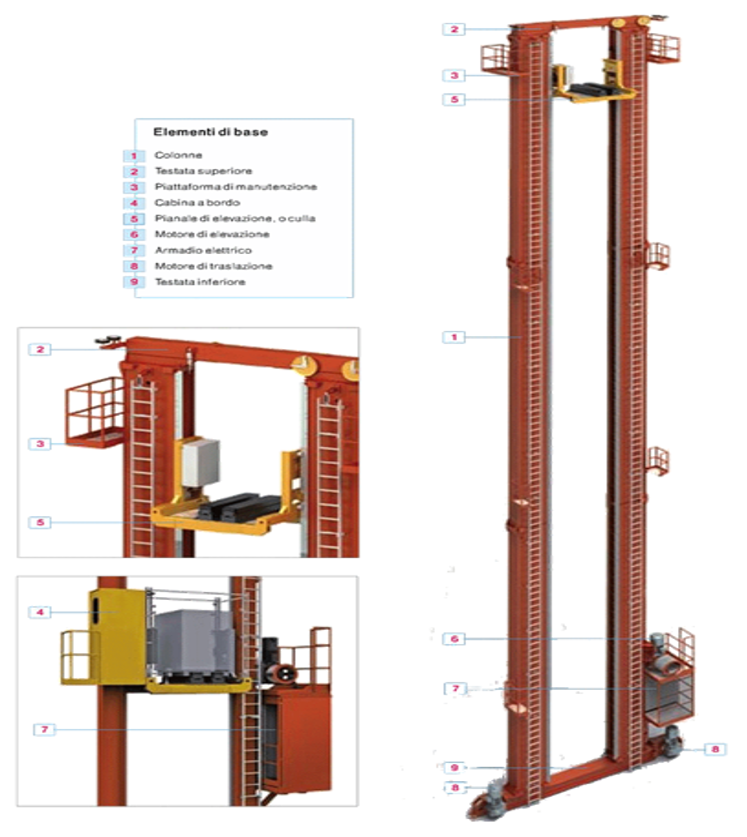
\includegraphics[width=0.4\linewidth]{assets/28.png}
    \caption{Trasloelevatore}\label{fig:trasloelevatori}
\end{figure}
%
\paragraph{Tipologie Strutturali e Scaffalature} La scelta strutturale è fondamentale in fase di progettazione:
\begin{itemize}
    \item \emph{Magazzino Tradizionale}: Le scaffalature sono installate all'interno di un edificio esistente. Si usa per altezze inferiori a 20-25 metri. Offre facilità di gestione antincendio e riutilizzabilità futura dell'immobile;
    \item \emph{Magazzino Autoportante}: Le scaffalature sostengono l'edificio stesso (pareti e copertura). Indicato per altezze elevate (>25 m, fino a 40 m). Richiede tempi di esecuzione ridotti ma presenta una gestione antincendio complessa.
\end{itemize}
Le scaffalature possono essere configurate in \textbf{semplice profondità} (accesso diretto a ogni UdC), \textbf{doppia profondità} (aumento della densità ma minore selettività) o \textbf{multi-profondità}.

%
\section{Logiche di Allocazione}
Per definire dove posizionare le merci, si utilizzano tre approcci principali:
\begin{enumerate}
    \item \textbf{Posti Condivisi (Random Storage)}: Qualunque articolo può occupare qualunque postazione libera. Massimizza l'utilizzo dello spazio;
    \item \textbf{Posti Dedicati (Dedicated Storage)}: Ogni articolo ha posizioni assegnate fisse. Comporta un utilizzo incompleto della scaffalatura;
    \item \textbf{Zone Dedicate (Class-based Storage)}: Gli articoli sono divisi in classi (Alta, Media, Bassa rotazione) e assegnati a zone specifiche per ottimizzare i tempi di prelievo (curva ABC).
          \begin{itemize}
              \item \emph{Nota sulla sicurezza}: Per evitare assembramenti (distanziamento sociale), è consigliabile distribuire i prodotti alto-rotanti uniformemente lungo le corsie.
          \end{itemize}
\end{enumerate}

%
\section{Cicli Operativi e Dimensionamento Dinamico}
La progettazione dinamica mira a calcolare i tempi di ciclo e il numero di macchine necessarie.
%
\paragraph{Tipologie di ciclo} Troviamo:
\begin{itemize}
    \item \textbf{Ciclo Semplice (CS)}: Il trasloelevatore preleva un'UdC dall'ingresso e la deposita (o viceversa per il prelievo), tornando poi alla base;
    \item \textbf{Ciclo Combinato (CC)}: Il trasloelevatore deposita un'UdC in entrata e, nello stesso viaggio, si sposta per prelevare un'UdC in uscita, ottimizzando il percorso.
\end{itemize}

%
\paragraph{Calcolo dei tempi (F.E.M. 9851)}
Per stimare le prestazioni, si modellizza il magazzino in coordinate temporali, trasformando le distanze in tempi ($T_l = L/v_l$ e $T_h = H/v_h$). La condizione ottimale di forma si ha quando il ``fattore di forma'' $h_l = T_{h} / T_{l}$ è pari a 1.

Secondo la norma F.E.M. 9851, si considerano due punti rappresentativi, $P_{1}$ e $ P_{2} $, per calcolare il tempo medio:

%
\subparagraph{Coordinate} $P_1 (1/5 L, 2/3 H)$ e $P_2 (2/3 L, 1/5 H)$
%
\subparagraph{Tempo Ciclo Semplice Medio}
\[
    T_m(CS) = t(P_1) + t(P_2) + 2t_{fissi}
\]
Dove $t(P)$ è il massimo tra il tempo di percorrenza orizzontale e verticale per raggiungere il punto.
%
\subparagraph{Tempo Ciclo Combinato Medio}
\[
    T_m(CC) = t(P_1) + t(P_1P_2) + t(P_2) + 4t_{fissi}
\]
Include il tempo di spostamento tra i due vani $t(P_1P_2)$.

%
\paragraph{Dimensionamento Macchine} Il numero di trasloelevatori (e quindi di corridoi) si calcola dividendo la potenzialità richiesta (PM) per i cicli/ora effettivi della macchina.
\begin{example}
    Performance tipiche: 30-40 cicli/h (semplice), 20-25 cicli/h (combinato) con efficienza 85-90\% .
\end{example}

%
\section{Sistemi per Piccole UdC}
Per picking, refilling e kitting di oggetti piccoli, si utilizzano tecnologie ``Materiali verso Operatore'' (Goods-to-Man).
%
\subsection{Magazzini Verticali (VLM - Vertical Lift Module)}
Strutture chiuse a sviluppo verticale con cassetti o vassoi movimentati da un elevatore interno verso una baia operatore.
\begin{itemize}
    \item \textbf{Vantaggi}: Riduzione impronta a terra (fino al 90\%), ergonomia, sicurezza, integrazione con WMS (riduzione errori e carta);
    \item \textbf{Prestazioni}: Fino a 190 picking/ora, altezze fino a 30m.
\end{itemize}
%
\subsection{Caroselli}
Possono essere:
\begin{itemize}
    \item \textbf{Verticali}: Ripiani rotanti (tipo paternoster).
    \item \textbf{Orizzontali}: Scaffalature rotanti orizzontalmente, adatte ad ambienti bassi (2-5 m).
\end{itemize}
%
\subsection{Miniload}
Simili ai trasloelevatori per pallet, ma progettati per cassette/cartoni. Elevata dinamica (fino a 500 cicli in/out per ora), altezze fino a 20m, adatti per stoccaggio intensivo in doppia profondità.
%
\subsection{Sistemi Shuttle}
Sistemi con navette indipendenti per ogni livello. Altissima produttività e flessibilità.
\begin{example}[Camozzi Automation]
    Possiede 40.000 locazioni, 73 shuttle, 500 cassette in/out per corsia.
\end{example}

\begin{table}
    \centering
    \begin{tabular}{llr}
        \toprule
        \textbf{Descrizione}          & \textbf{Equazione / Formula}                 & \textbf{Rif. / Unità}      \\
        \midrule
        Tempo percorrenza orizzontale & $T_l = L / v_l$                              & Coord. temp.               \\
        Tempo percorrenza verticale   & $T_h = H / v_h$                              & Coord. temp.               \\
        Fattore di forma ideale       & $h_l = T_h / T_l = 1$                        & Adimensionale              \\
        Punto caratteristico $P_1$    & $(1/5 L, 2/3 H)$                             & F.E.M. 9851                \\
        Punto caratteristico $P_2$    & $(2/3 L, 1/5 H)$                             & F.E.M. 9851                \\
        Tempo Medio Ciclo Semplice    & $T_m(CS) = t(P_1) + t(P_2) + 2t_{fissi}$     & $t(P) = \max(t_x, t_y)$    \\
        Tempo Medio Ciclo Combinato   & $T_m(CC) = T_m(CS) + t(P_1P_2) + 2t_{fissi}$ & Include inter-vano         \\
        Numero Trasloelevatori        & $N = PM / \text{Cicli}_{eff}$                & $PM = \text{Potenzialità}$ \\
        Indice di Accesso (Picking)   & $I_A = \frac{Popularity}{Volume}$            & $\frac{accessi}{m^3}$      \\
        \bottomrule
    \end{tabular}
    \caption{Riepilogo delle formule per il dimensionamento dei sistemi di stoccaggio e picking.}\label{tab:formule_magazzino}
\end{table}


%
\subsection{AutoStore}
Sistema ad altissima densità composto da una griglia cubica autoportante. I robot corrono sulla parte superiore della griglia, prelevando le cassette dall'alto (``digging'').

È flessibile, scalabile, ottimo per e-commerce e ricambistica (es. caso Malò). Gestisce decine di migliaia di referenze in spazi ridotti.

%
\section{Criteri di Scelta: Analisi ABC Incrociata}
La scelta del sistema di stoccaggio corretto si basa sull'incrocio tra la Quantità a stock (Volume) e la Frequenza di movimentazione.
\begin{itemize}
    \item \emph{Alta quantità / Bassa frequenza}: Sistemi ad alta densità come Drive-in o Catasta.
    \item \emph{Alta quantità / Alta frequenza}: Sistemi a gravità o trasloelevatori con scaffali a gravità/doppia profondità.
    \item \emph{Bassa quantità / Alta frequenza}: Scaffali serviti da carrelli o transpallet (picking manuale veloce).
    \item \emph{Media quantità / Media frequenza}: Scaffali serviti da trasloelevatori in semplice profondità o carrelli trilaterali.
\end{itemize}
Vedi figura \ref{fig:abc}.

\begin{figure}
    \centering
    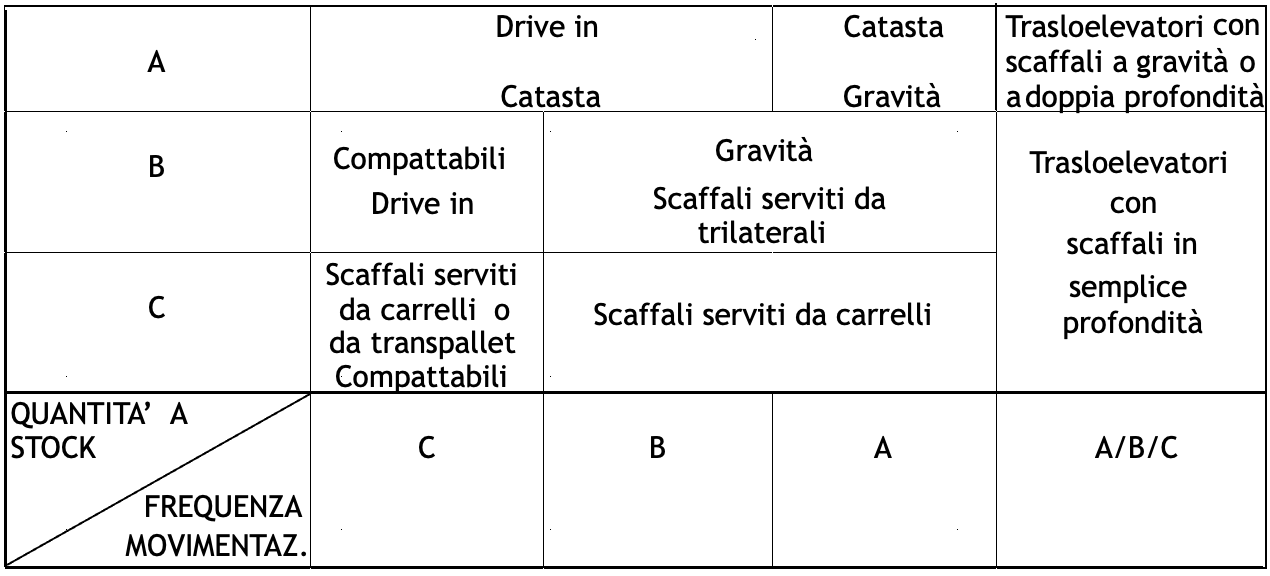
\includegraphics[width=0.63\linewidth]{assets/Screenshot 2026-01-26 at 16.47.35.png}
    \caption{Analisi ABC}\label{fig:abc}
\end{figure}